\section{Interpolation}\label{interpolation}

To get smooth transitions of parameters between keyframe there are used
interpolation functions, which calculates intermediate values. There is no need
for manual change of camera position and fractal parameters for every animation
frame. Limited number of keyframes is enough to define good looking animation.

\subsection{Interpolation types}\label{interpolation-types}

There are implemented several interpolation functions:

\begin{enumerate}
	
	\item None
	
	\item Linear
	
	\item Linear angle
	
	\item Akima
	
	\item Akima angle
	
	\item Catmul-Rom
	
	\item Catmul-Rom angle degrees
	
\end{enumerate}

\begin{samepage}
	
	The chart bellow shows comparison between different interpolation modes
	
	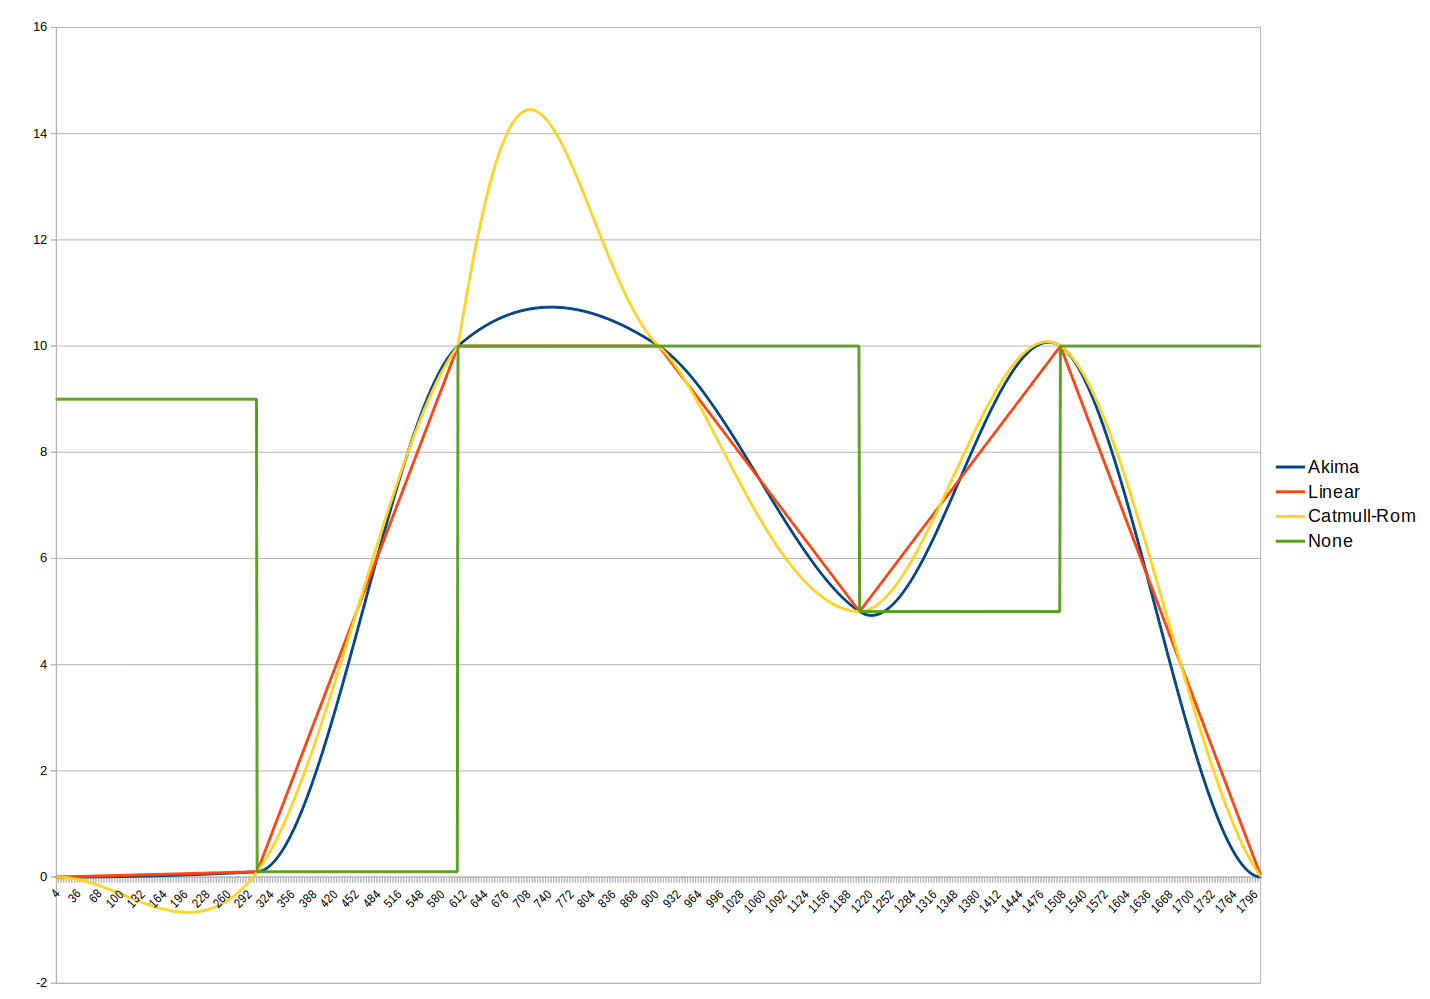
\includegraphics[width=1.0\linewidth]{img/manual/media/interpolations}
	
	As it is visible, depending which interpolation function will be used, the
	final result of animation will be different.
	
\end{samepage}

\subsubsection{Interpolation - None}\label{interpolation-none}

Parameter is not interpolated. After every keyframe the value of parameter will
have step change. This mode can be used with boolean values or with variables
which have to be kept at constant levels for some number of keyframes.

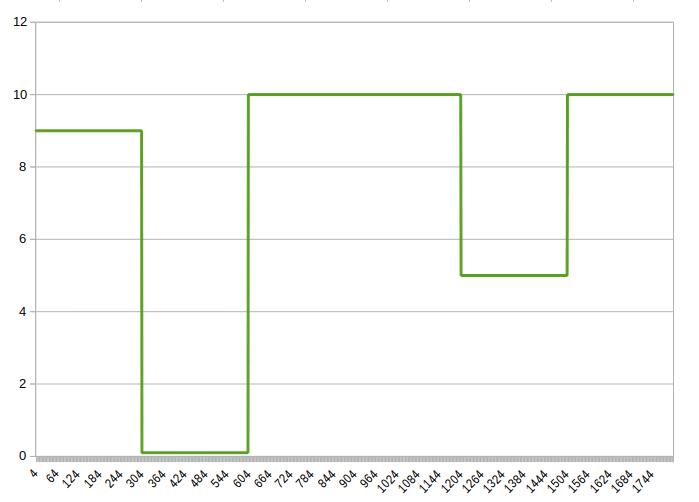
\includegraphics[width=0.5\linewidth]{img/manual/media/interpolation_none}

\subsubsection{Interpolation - Linear}\label{interpolation-linear}

Value of parameter is interpolated using linear functions.

\[ y(x) = y_i + (x - x_i) \frac{y_{i+1} - y_i}{x_{i+1} - x_i}\] \[x_i  \leq x
\leq x_{i+1}\]

Changes of parameters are easy to predict. There are no overshoots. This
interpolation mode is good for fractal parameters and material properties. It's
not recommended to use it for camera or objects movement paths, because of rapid
changes of speed.

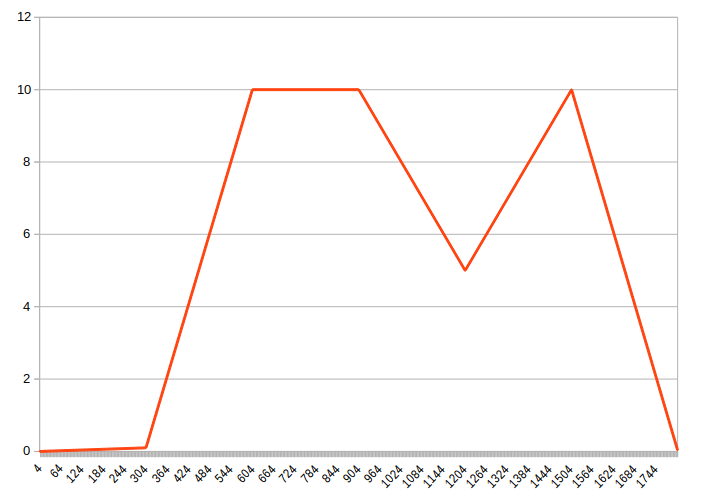
\includegraphics[width=0.5\linewidth]{img/manual/media/interpolation_linear.png}

\subsubsection{Interpolation - Linear angle}\label{interpolation-linear-angle}

This interpolation mode works like \emph{Linear}, but is prepared of angular
parameters. If value exceed 360 degrees, then will go back to zero.

\subsubsection{Interpolation - Akima}\label{interpolation-akima}

The Akima interpolation is a continuously differentiable sub-spline
interpolation. It is built from piecewise third order polynomials.

\[ y(x) = a_0 + a_1 (x - x_i) + a_2 (x - x_i)^2 + a_3 (x - x_i)^3\] \[x_i  \leq
x \leq x_{i+1}\]

This interpolation method is very good for most of animated parameters. It can
be used for camera and target animation and for many other parameters which
should be animated in smooth way.

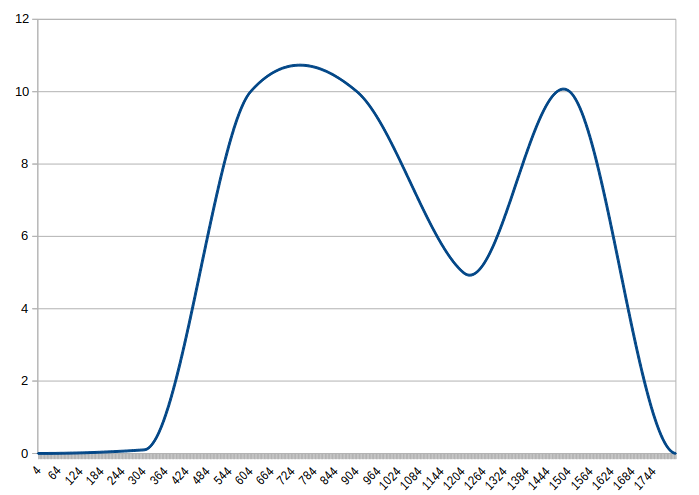
\includegraphics[width=0.5\linewidth]{img/manual/media/interpolation_akima.png}

\subsubsection{Interpolation - Akima angle}\label{interpolation-akima-angle}

This interpolation mode works like \emph{Akima}, but is prepared of angular
parameters. If value exceed 360 degrees, then will go back to zero.

\subsubsection{Interpolation - Catmul-Rom}\label{interpolation-catmul-rom}

Catmull-Rom splines are cubic interpolating splines formulated such that the
tangent at each point $ y_i(x_i) $ is calculated using the previous and next
point on the spline.

\[ y(x) = 0.5 \begin{bmatrix} 1 & x-x_i & (x-x_i)^2 & (x-x_i)^3\end{bmatrix}
\begin{bmatrix} 0 & 2 & 0 & 0 \\ -1 & 0 & 1 & 0 \\ 2 & -5 & 4 & -1 \\ -1 & 3 &
-3 & 1 \\ \end{bmatrix} \begin{bmatrix} y_{i-1} \\ y_i \\ y_{i+1} \\ y_{i+2}
\end{bmatrix} \]

This interpolation gives very smooth results. Animated objects looks like made
of springy materials. It can be used to animate fractal parameters and also
camera path. This interpolation can produce oscillations, so has to be used
carefully. As it is visible on the chart below, values went below zero when all
of keyframe values were higher than zero.

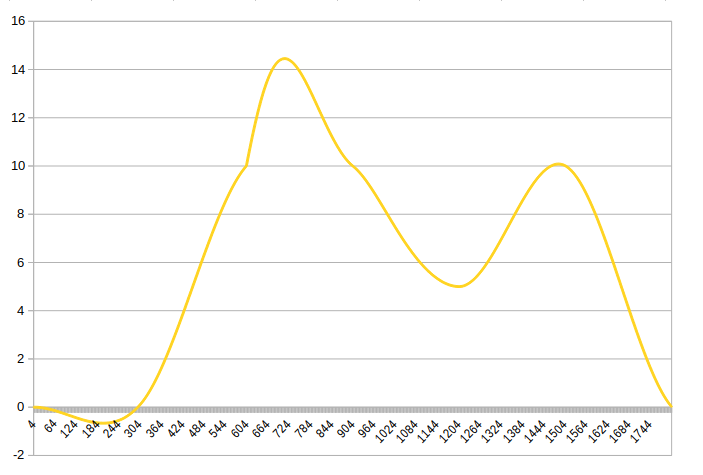
\includegraphics[width=0.5\linewidth]{img/manual/media/interpolation_catmulrom.png}

\subsubsection{Interpolation - Catmul-Rom
	angle}\label{interpolation-catmul-rom-angle}

This interpolation mode works like \emph{Catmul-Rom}, but is prepared of angular
parameters. If value exceed 360 degrees, then will go back to zero.

\subsection{Catmul-Rom / Akima interpolation -
	Advices}\label{catmul-rom-akima-interpolation---advices}

\subsubsection{Collision}\label{collision}

Fast approaching the obstacle may cause inadvertent drag to the camera towards
the center of the object. 

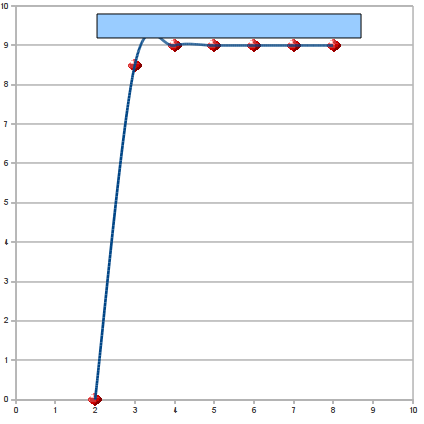
\includegraphics[width=0.4\linewidth]{img/manual/media/catmull-rom_collision.png}

It is recommended to maintain the principle that one
keyframe does not reduce the distance to the object more than 5-times.

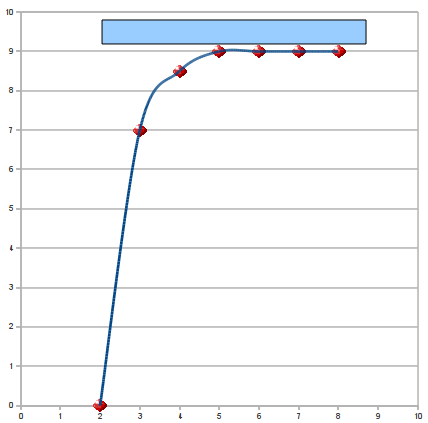
\includegraphics[width=0.4\linewidth]{img/manual/media/catmull-rom_no_collision.png}


\subsubsection{Fly through the gap}\label{fly-through-the-gap}

It is recommended to place a keyframe at the point where the camera flies
through the gap

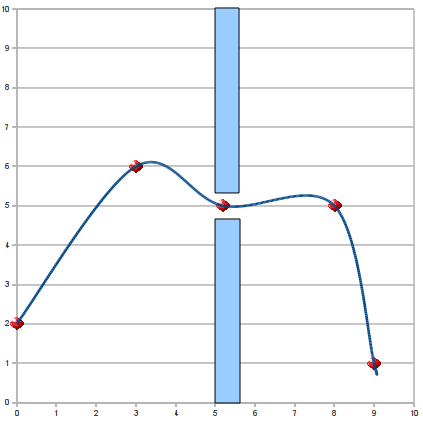
\includegraphics[width=0.4\linewidth]{img/manual/media/catmull-rom_hole.png}

\subsubsection{Proper conduct cameras between
	objects}\label{proper-conduct-cameras-between-objects}

Image below shows how keyframes should be located between objects to avoid collisions caused by interpolation functions.  

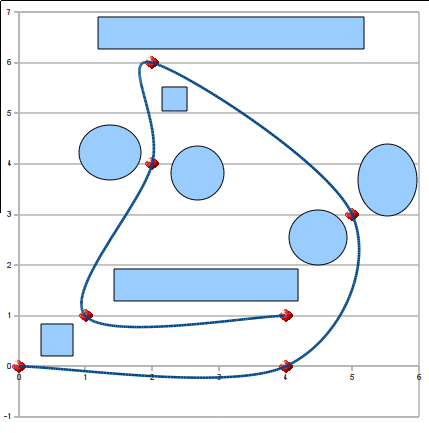
\includegraphics[width=0.4\linewidth]{img/manual/media/catmull-rom_example.png}

\subsection{Changing interpolation types}\label{changing-interpolation-types}

To change the interpolation algorithm, right click on the parameter list and the
options appear. In this example the main\_formula\_weight parameters have been
changed from Akima to Linear. Interpolation type is color coded e.g. Linear
parameters are highlighted in grey.

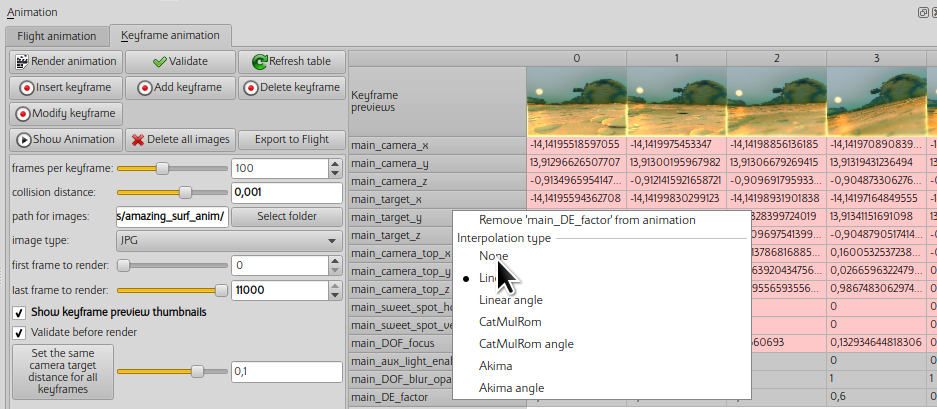
\includegraphics[width=\linewidth]{img/manual/media/change_interpolation_type.png}
